\newpage
\section{Steuerstrukturen}
\subsection{basics}
Die Wichtigen Steuerstrukturen in einer Auflistung(mit korrekter Syntax) 

\begin{lstlisting}[language = c]
#include <stdio.h>//inkludiert stdio.h(brauchts hier nicht)
int main() //Programmaufruf
{
    if(<Bedingung>)
    {
        ;//Anweisung wenn wahr
    }
    else
    {
        ; //Anweisung wenn Falsch
    }

    while(<Bedingung>)//wenn Anweisung nicht wahr zu beginn wird Schleife nicht betreten
    {
        ;//mache so lange bis Bedingung falsch
        continue;//springe in den naechsten Schleifendurchlauf
    }

    do//mindestens 1 Durchlauf gibt es
    {
        ;//mache so lange bis Bedingung falsch
    } while(<Bedingung>);

    for(int i = 0;<Bedingung>,i++)// int I wird nur einmal initialisiert und i wird immer nach dem schleifendurchgang initialisiert
    {
        ;//mache so lange bis Bedingung falsch
    }

    case(<variable>)//springe basierend auf der Variable
    {
        case 0://springt hier wen var = 0
            break;//ohne break wuerde switch hier weiterlaufen
        case 1 ... 4 : //range von 1-4
            break;
        default://sonst trifft nichts zu
            break;
    }

    return <wert>;//Return einer Funktion
    return 0;//Programm korrent durchlaufen
    return 1;//programm nicht korrekt durchlaufen Fehlercode 1    
}
\end{lstlisting}

\subsubsection{Sprunganweisungen}

\begin{itemize}[itemsep=1pt, parsep=0pt]
    \item \textbf{break} \newline (do)while, for, switch abbrechen.
    \item \textbf{continue} \newline bei (do)while und for in den nächsten Schleifendurchgang springen.
    \item \textbf{return} \newline aus Funktion an aufrufende Stelle zurückspringen
    \item \textbf{goto} \newline innerhalb einer Funktion an eine Marke (Label) springen(sind nie gerechtfertigt verwendet)
\end{itemize}

\subsubsection{GoTo}

Ein mit einem goto kann man \textbf{innerhalb einer Funktion} zu einer Marke Springen. Das kann sehr komfortabel sein, führt aber fast immer zu sehr schwer lesbaren Code. Möglichst nie verwenden.\newline
Ein Beispiel:

\begin{lstlisting}[language = c]
#include <stdio.h>

int func()
{
    printf("Do func Stuff\n");
inFunc: //hindert den normalen Programmablauf nicht
    return 0;
}

int main()
{
    printf("Anfang von main\n");
    func();
    goto hell;//Sprung zur marke hell
    printf("Sollte nie ausgegeben werden\n");
hell: //Marken sind so indentiert
    printf("spring hierher\n");

    goto inFunc;//Funktioniert nicht! da out of scope
    
    return 0;
}
\end{lstlisting}

\subsection{Funktionen}

Funktionen ist eine Zusammenfassung von Anweisungen, die ein und Ausgabewerte haben kann.\newline
\textless{}returnType\textgreater{} \textless{}functionName\textgreater{} (\textless{}paramType1\textgreater{} \textless{}paramName1\textgreater{}, \textless{}paramType2\textgreater{} \textless{}paramName2\textgreater{}, … );\newline
Wenn eine Funktion aufgerufen wird, müssen immer \textbf{alle} Parameter mitgegeben werden.\newline

\subsubsection{Funktionsprototyp}

Funktionen werden typischerweise weit oben im Quelltext definiert, als Funktionsprototyp. Der Funktionsprototyp legt das Interface der Funktion fest (Meist in .h Files festgelegt). Er \textbf{muss} verwendet werden, wenn die Funktion vor Definition verwendet werden möchte.

\begin{lstlisting}[language = c]
int myFunc(int input1, int input2,...);//Funktionsprototyp
int myfunc(int input1)//direkte definition
{
    Return 0;
}
\end{lstlisting}
Der Parametername kann zwischen Prototyp und Definition unterschiedlich sein, ist aber nicht empfohlen.

\subsubsection{Void}

Void als Returntyp heisst das kein Wert zurückgegeben wird.\newline
Return darf verwendet werden, aber es darf kein Wert hinterlegt werden.\newline
Void als Parameter heisst das kein Parameter übergeben werden kann. Es kann auch weggelassen werden.

\subsection{Pointer auf Funktionen}

Pointer können auch auf Funktionen definiert werden zum z.B. zur Laufzeit dynamische Programmabläufe zu realisieren.\newline
Syntax: int (*name)(int,int);

\begin{itemize}[itemsep=1pt, parsep=0pt]
    \item \textbf{int} : Return Typ der funktion
    \item \textbf{(*name)} : name des Pointer
    \item \textbf{(int,int)} : aufrufparameter(hier 2*int)

\end{itemize}

bsp:

\begin{lstlisting}[language = c]
int compare (int a, int b) { ... }
int main() 
{
    int (*ptr)(int, int);//pointer definieren
    ptr = &compare; // Zuweisen der Funktionsadresse
    ptr = compare; // tut dasselbe, d.h. man darf das & bei Funktionen auch weglassen
    printf("Vergleich liefert: ", (*ptr)(37, 12)); // Funktionspointer wird dereferenziert
}
\end{lstlisting}

\subsection{Funktionen : Iteration und Rekursion}

\begin{itemize}[itemsep=1pt, parsep=0pt]
    \item Rekursion: eine Funktion ruft sich selbst auf.
    \item Iteration: Algorithmus enthält Abschnitte, die innerhalb einer Ausführung mehrfach durchlaufen werden (Schleife)
    \item Jeder rekursive Algorithmus kann auch iterativ formuliert werden
    \item Die rekursive Form kann eleganter sein, ist aber praktisch immer ineffizienter als die iterative Form.
    \item Das Abbruchkriterium ist bei beiden Formen zentral
\end{itemize}

\subsubsection{Anwendungen}
\begin{itemize}[itemsep=1pt, parsep=0pt]

    \item Backtracking-Algorithmen z.B. Finden eines Weges durch ein Labyrinth (zurück aus Sackgasse und neuen Weg prüfen)
    \item Implementierung rekursiv definierter mathematischer Funktionen (z.B. Fakultätsfunktion)
    \item \textbf{Achtung}: der Speicherbedarf ist bei Rekursion schwer abzuschätzen. Rekursive Funktionen sind deshalb insbesondere bei der Embedded Programmierung zu vermeiden.
    \item \textbf{Achtung}:jede Instanz einer rekursiv gerufenen Funktion besitzt ihre eigenen, unabhängigen Variablenkopien. Ausnahme: static-deklarierte lokalen Variablen
    \item Indirekte Rekursion ist unbedingt zu vermeiden Diese kommt z.B. zustande, wenn sich zwei oder mehrere Funktionen wechselseitig oder im Kreis aufrufen
\end{itemize}

\subsubsection{Beispiel}

Hier diese Folgenden Funktionen berechnen beide die Fakultät einer Zahl.\\

\noindent
\begin{minipage}[t]{0.5\columnwidth}
Fakultät \textbf{Iterativ}
\begin{lstlisting}[language = c]
uint64 fak(uint64 n)
{
    uint64 val = 1;
    for (int i = 2; i <= n; ++i)
    {
        val = val * i;
    }
    return val;
}


\end{lstlisting}
\end{minipage}
\begin{minipage}[t]{0.5\columnwidth}
Fakultät \textbf{rekursiv}
\begin{lstlisting}[language = c]
uint64 fak(uint64 n)
{
    if (n > 1)
    {
        return n * fak(n-1);
    }//Erneuter Aufruf der Funktion fak
    else
    {
        return 1;
    }
}
\end{lstlisting}
\end{minipage}
\subsection{Operatoren}

Operatoren haben eine Priorität, welche aussagt in welcher Reihenfolge die Befehle ausgeführt werden. Haben Operatoren dieselbe Priorität besagt die Assoziativität in welcher Reihenfolge ausgewertet wird.\newline

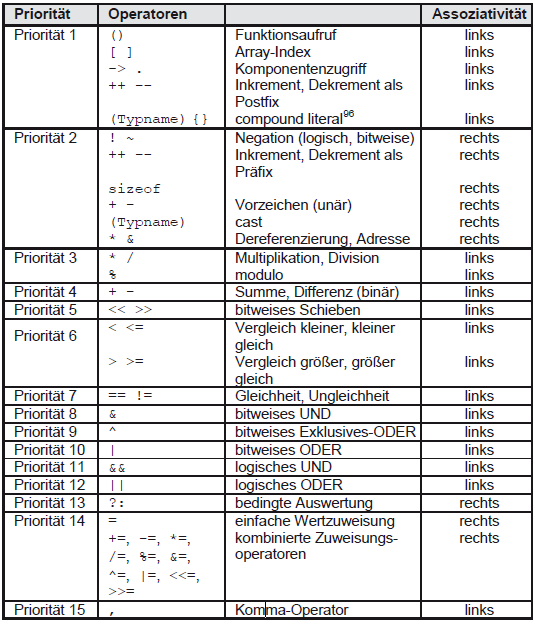
\includegraphics[width=1\columnwidth]{Pictures/Operators.png}

\subsubsection{Sizeof}

Sizeof gibt die Grösse(in Bytes) eines Datentyp/array's zurück.

\begin{lstlisting}[language = c]
sizeof(char);//immer 8
sizeof(myArray)/sizeof(myArray[0]);//liefert die groesse eines Arrays
\end{lstlisting}

\subsubsection{Mini if}

Der ternäre Operator braucht 3 Argumente. Je nach Wahrheitswert wird, nach links oder rechts gesprungen.
\begin{lstlisting}[language = c]
<Bedinging>?"wahr":"unwahr";

return myInt==3?5:0;//Wenn myInt ist 3, wird 5 dem return Operator uebergeben. Ansonsten wird 0 uebergeben

\end{lstlisting}

